\subsection{Experimental setup}
The experiments were executed in a Mac Book Pro with the following characteristics: 2,6 GHz Intel Core i5, 8 GB 1600 MHz DDR3 memory and 256 GB of storage.

\subsection{Analysis}
Data set coming from previous steps are used as an input for the calculations in the analysis. These are some of the most relevant features:
\begin{itemize}
    \item system\_time - timestamp of the recording
    \item cell\_loc - event's approximated location
    \item gps\_loc - event's GPS location, considered as ground truth
\end{itemize}

The analysis phase is executed with a following steps. For each date between 2018-03-12 and 2018-03-16 we do the following:
\begin{enumerate}
    \item Import input data to pySpark DataFrame from Parquet files
    \item Calculate Euclidean distance measure on trajectories
    \item Calculate edit distance distance measure on trajectories
\end{enumerate}

For the whole input data set we also do the following:
\begin{enumerate}
   \item Generate and display histograms on pairwise distances
    \item Calculate descriptive statistics on pairwise distances:
        \begin{itemize}
            \item min
            \item max
            \item sum
            \item mean
            \item standard deviation
        \end{itemize}
    \item Visualize on map
\end{enumerate}
    
\subsection{Results}
Looking at the histogram of pairwise spatial distances between the trajectories in Figure\ref{fig:hist} we can say that the majority of the events were positioned with more than 1.5 kilometers uncertainty. Roughly the other half of events were localized with 500 to 1000 meters accuracy, which is still too large for reliable geo-positioning.

We expect that the quality of positioning can be significantly improved by using more accurate and robust information about cell towers.

\begin{figure}[h]
    \centering
    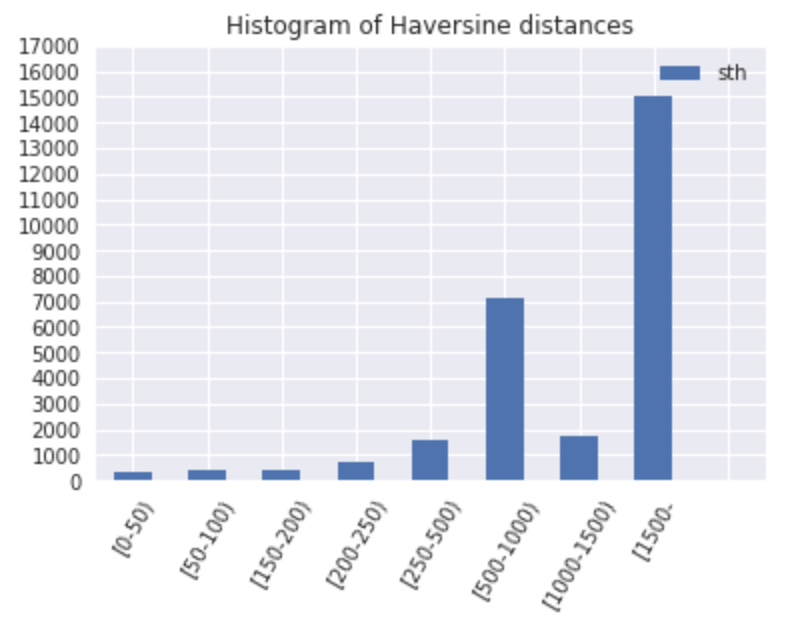
\includegraphics[width=0.5\textwidth]{images/hist.png}
    \caption{Histogram of pairwise spatial distance of the point in trajectories}
    \label{fig:hist}
\end{figure}


This result can change depending on individual customer's mobile usage habits, network characteristics, cell map data source and the customer's geographical position.

From the results in Table \ref{tab:distances}, we can conclude that the overall positioning needs a lot of improvement. The reason why both measures are this high is the fact that the square operation in Euclidean distance tends to penalize large distances. 

From Table \ref{tab:dist_stats} we see the maximum distance is only around 1.65 kilometers, which does not seem to be extremely high, but this is only because the observations with higher distances are filtered out when joining the CDR and cellmap data sets. 
The 1.4 meters minimum distance is very low, so it means that for some observations the positioning was very accurate. This would probably happen when the user was very close to the cell tower they connected to. The standard deviation of distances is 456.52 meters, which means that the distribution of distances is fat.

CORRELATION; GRAPH of DISTANCE measures, also save as a notebook
\begin{table}[h]
    \centering
    \begin{tabular}{|l|c|c|}
        \hline
        \textbf{Date} & \textbf{Euclidean distance} & \textbf{Edit distance}\\
        \hline 
        2018-03-01 & ??? & ?? \\
        \hline 
        2018-03-02 & ??? & ?? \\
        \hline 
        2018-03-03 & ??? & ?? \\
        \hline 
        2018-03-04 & ??? & ?? \\
        \hline 
        2018-03-05 & ??? & ?? \\
        \hline 
        2018-03-06 & ??? & ?? \\
        \hline 
        2018-03-07 & ??? & ?? \\
        \hline 
        2018-03-08 & ??? & ?? \\
        \hline 
        2018-03-09 & ??? & ?? \\
        \hline 
        2018-03-10 & ??? & ?? \\
        \hline 
        2018-03-11 & ??? & ?? \\
        \hline 
        2018-03-12 & ??? & ?? \\
        \hline 
        2018-03-13 & ??? & ?? \\
        \hline 
        2018-03-14 & ??? & ?? \\
        \hline 
        2018-03-15 & ??? & ?? \\
        \hline 
        2018-03-16 & ??? & ?? \\
        \hline
    \end{tabular}
    \caption{Distance measures during the studied period}
    \label{tab:distances}
\end{table}

\begin{table}[h]
    \centering
    \begin{tabular}{|l|c|}
        \hline
        \textbf{Statistic} & \textbf{Value} \\
        \hline 
        count & $27398$ \\
        \hline
        min(dist) &  $1.40$\\
        \hline
        max(dist) &   $1652.51$\\
        \hline
        avg(dist) &  $839.04$\\
        \hline
        stddev(dist) &  $456.52$\\
        \hline
    \end{tabular}
    \caption{Descriptive statistics of Haversine distances (in meters)}
    \label{tab:dist_stats}
\end{table}

When the user is located between several cell towers, the connection can be passed from one tower to another depending on network traffic fluctuations and other factors. This phenomenon is often referred to as cell tower ping-pong handover. It can however be used for improving positioning and identifying points-of-interest (POIs). As seen in Figure \ref{fig:ping-pong}, the phone connects to a cell tower and to another one and then back again to the previous one. Without knowing the actual GPS position we could better approximate the location of the customer using the ping-pong handover schema.

\begin{figure}[h]
    \centering
    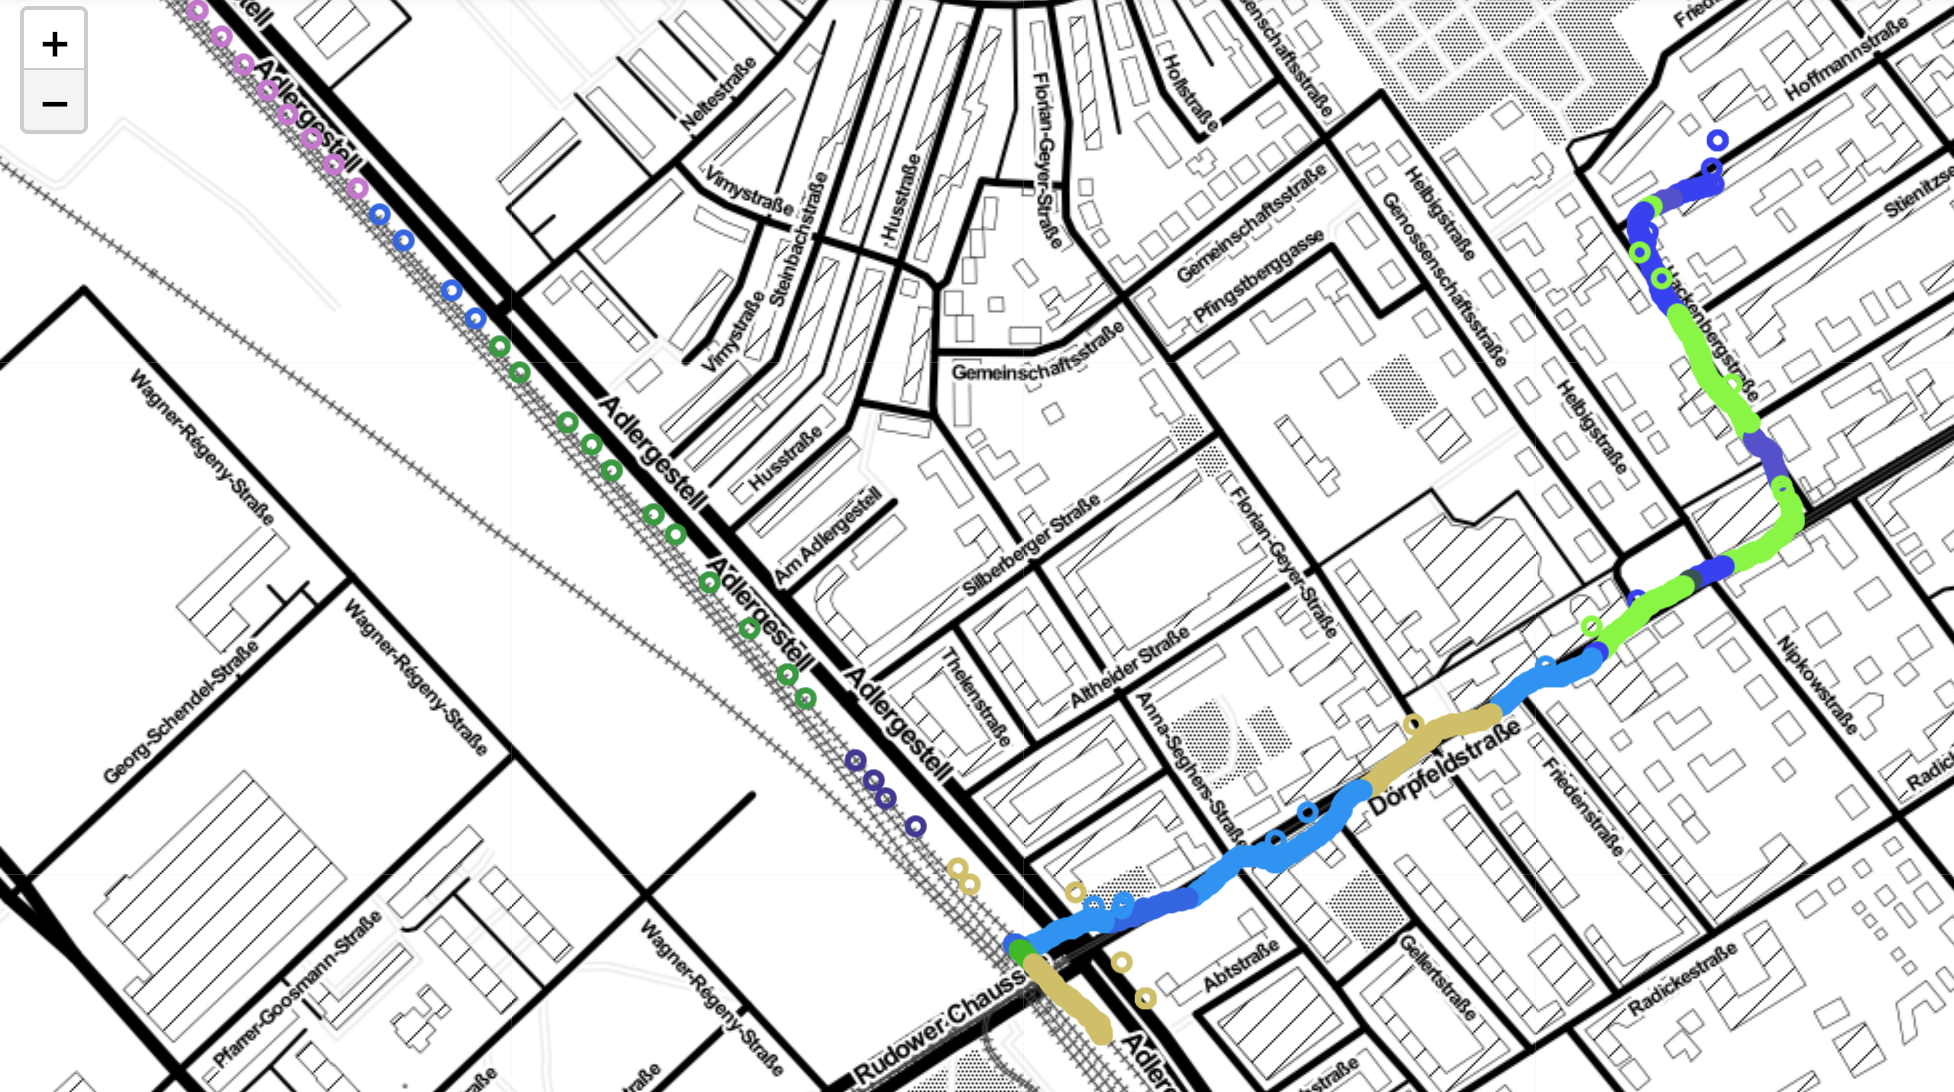
\includegraphics[width=0.5\textwidth]{images/ping-pong.png}
    \caption{Cell ping-pong handover problem, GPS points color based on the connected cell tower}
    \label{fig:ping-pong}
\end{figure}

This method can be further improved if we take into account the angle of the antennas on the cell towers. If we know which antenna is getting the signal, we can guess the direction of the transmitting cell phone and the signal strength can give an approximation of how far away it is. This method is called cell tower triangulation and can be quite accurate in rural regions with more cell towers. However the information about the angles of the antennas and the signal strength can be outdated or even missing therefore it is not always applicable. In this analysis we did not obtain robust data about the positions of the antennas and the signal strength for each CDR event.

Positioning could be improved by reconstructing trajectories considering the road network of Berlin and the potential speed of the movement instead of simply assigning the the cell location from the cell map data.

We identified three major external factors defining the accuracy of the positioning:
\begin{itemize}
    \item individual mobile usage habits affecting the sparsity of CDR data,
    \item geographical location, as rural and urban areas has different cell size and therefore location defines the accuracy of cell tower localization and
    \item cellular network characteristics that define the overall data quality and the available attributes in the CDR data-set.
\end{itemize}
